\documentclass[11Pt,t,compress]{beamer}
%------------------------------------------------------------
%\documentclass[handout]{beamer}
%\usepackage{pgfpages}
%\pgfpagesuselayout{2 on 1}[a4paper,border shrink=5mm] %| handout:0
%------------------------------------------------------------

\usepackage{graphicx}
\usepackage{amsmath}
\usepackage{amssymb,amsfonts}
\usepackage[latin1]{inputenc}
\usepackage{colortbl}
\usepackage{lmodern}
\usepackage{ae}
\usepackage{pict2e}
\usepackage{alltt}
\usepackage{psfrag}
\usepackage{wasysym}
\usepackage{rotating}
\usepackage{calc}
\usepackage{Util}
\usepackage{eurosym}
\usepackage{mathtools}
\usepackage{color}
\usepackage{soul}
\usepackage{cancel}
\usepackage{multirow}
\usepackage{bm,xcolor}
\usepackage{amsthm,epstopdf,dsfont}

\theoremstyle{definition}
\newtheorem{Thrm}{Theorem}
\newtheorem{Lmm}{Lemma}
\newtheorem{Exm}{Example}
\newtheorem{Sol}{Solution}
\newcommand\hcancel[2][black]{\setbox0=\hbox{$#2$}
	\rlap{\raisebox{.45\ht0}{\textcolor{#1}{\rule{\wd0}{1pt}}}}#2} 
%\usepackage{movie15}
%---------------- Struktur und Themes ----------------
%
\mode<presentation>
{
    \usefonttheme[onlysmall]{structurebold}
    \usefonttheme[onlymath]{serif}
    \useinnertheme{rectangles}
    \useoutertheme{split}
    \usecolortheme{orchid}
    \usecolortheme{whale}
}

\setbeamerfont{headline}{size=\Tiny}

%----------------  Definition Farben ----------------
\definecolor{UB_Blau_histo}{RGB}{51,153,255}
\definecolor{UB_Blau1}{RGB}{230,235,250}
\definecolor{UB_Blau11}{RGB}{230,235,250}
\definecolor{UB_Blau2}{RGB}{186,204,238}
\definecolor{UB_Blau3}{RGB}{163,189,232}
\definecolor{UB_Blau33}{RGB}{163,189,232}
\definecolor{UB_green}{RGB}{251,255,251}
\definecolor{midgreen}{RGB}{60,200,20}
\definecolor{lightgreen}{RGB}{190,247,175}
\definecolor{lightyellow}{RGB}{255,255,147}
\definecolor{weiss}{RGB}{255,255,255}
\definecolor{grau}{gray}{.90}
\definecolor{grau2}{gray}{.95}
\definecolor{blue1}{rgb}{0.32,0.93,0.91}
\definecolor{blue2}{rgb}{0.18,0.59,1.00}
\definecolor{lightblue2}{rgb}{0.85,0.85,1.00}
\definecolor{lightgreen}{rgb}{0.80,1.00,0.80}
\definecolor{lightblue1}{rgb}{0.80,1.00,1.00}
\definecolor{green2}{rgb}{1.00,1.00,0.00}
\definecolor{verylightgray}{rgb}{0.90,0.90,0.90}
\definecolor{lightred}{rgb}{0.90,0.40,0.40}
\definecolor{lightred2}{rgb}{0.80,0.20,0.20}

\definecolor{col1}{RGB}{0,255,0}
\definecolor{col2}{RGB}{102,204,0}
\definecolor{col3}{RGB}{255,255,0}
\definecolor{col4}{RGB}{255,128,0}
\definecolor{col5}{RGB}{255,0,0}

\definecolor{rot}{RGB}{255,200,200}
\definecolor{hellrot}{RGB}{255,230,230}

\definecolor{gruen}{RGB}{210,240,200}
\definecolor{hellgruen}{RGB}{230,247,225}
\definecolor{e_gruen}{RGB}{0,96,0}
\definecolor{ex_gruen}{RGB}{0,128,0}

\definecolor{gold}{RGB}{255,230,153}
\definecolor{hellgold}{RGB}{255,247,221}

\definecolor{hellblau}{RGB}{212,224,244}

\definecolor{blau}{RGB}{30,50,255}
\definecolor{dunkelblau}{RGB}{51,51,178}

\setbeamercolor*{palette primary}{use=structure,fg=black,bg=UB_Blau1!}
\setbeamercolor*{palette secondary}{use=structure,fg=white,bg=structure.fg!75!black}
\setbeamercolor*{palette tertiary}{use=structure,fg=white,bg=structure.fg!50!black}
\setbeamercolor*{palette quaternary}{fg=black,bg=white}

\setbeamercolor{block title}{use=structure,fg=black,bg=UB_Blau33}
\setbeamercolor{block body}{parent=normal text,use=block title,bg=UB_Blau11}

\setbeamercolor{block body example}{parent=normal text,use=block title,bg=UB_green}

\setbeamercolor{section in head/foot}{parent=palette quaternary}
\setbeamercolor{subsection in head/foot}{parent=palette quaternary}

\setbeamercolor{author in head/foot}{parent=palette primary}
\setbeamercolor{title in head/foot}{parent=palette primary}

%----------------  Seitenzahlen ----------------
%
\defbeamertemplate*{slidenumber}{framenumber} {\insertframenumber}
\defbeamertemplate{slidenumber}{totalframenumber} {\insertframenumber\,/\,\inserttotalframenumber}
\defbeamertemplate{slidenumber}{pagenumber} {\insertpagenumber}
\defbeamertemplate{slidenumber}{totalpagenumber} {\insertpagenumber\,/\,\insertpresentationendpage}

\setbeamertemplate{navigation symbols}{}

\defbeamertemplate*{footline}{slidenumber right}
{
  \leavevmode
  \hbox{\begin{beamercolorbox}[wd=\paperwidth,ht=2.5ex,dp=1.125ex,leftskip=.3cm,rightskip=.3cm]{title in head/foot}
    \usebeamerfont{title in head/foot}
    \insertshorttitle \hfill \insertshortauthor \hfill \usebeamertemplate{slidenumber}
  \end{beamercolorbox}}
}

\newcommand{\real}{\mathbb{R}}
\newcommand{\R}{\mathbb{R}}
\newcommand{\realp}{\mathbb{R}_{>0}}
\newcommand{\realzp}{\mathbb{R}_{\ge 0}}
\newcommand{\integer}{\mathbb{Z}}
\newcommand{\integerp}{\mathbb{Z}_{>0}}
\newcommand{\integerzp}{\mathbb{Z}_{\ge 0}}
\newcommand{\argmin}{\mathrm{arg\,min}}

\newcommand{\explain}[2]{\underset{\mathclap{\overset{\uparrow}{#2}}}{#1}}
\newcommand{\explainup}[2]{\overset{\mathclap{\underset{\downarrow}{#2}}}{#1}}


\setbeamercovered{dynamic}

%Logo Position neu, oben rechts:
%\pgfdeclareimage[height=0.8cm]{uni}{images/logo_NT}
%\logo{\pgfuseimage{uni}}

\makeatletter
\setbeamertemplate{frametitle}{%
  \begin{beamercolorbox}[wd=\paperwidth,leftskip=.5cm,% von links her eingeschoben
       rightskip=-1mm,vmode,sep=0.0001cm]{frametitle}
%  \begin{beamercolorbox}[sep=0.3cm,#1,wd=\the\@tempdima]{frametitle}
    \usebeamerfont*{frametitle}%
        %\vbox{}%\vskip-0ex%
    \strut\insertframetitle\strut\hfill\parbox{1.5cm}{\insertlogo}% xx cm nach links eingeschoben
      \ifx\insertframesubtitle\@empty\else\par%
        {\usebeamerfont*{framesubtitle}{%
         \usebeamercolor[fg]{framesubtitle}%
         \insertframesubtitle}\strut\par}%
      \fi%
  \end{beamercolorbox}}
\makeatother
\setbeamertemplate{sidebar right}{% hier kein logo
  \vfill%
  \vskip2pt%
  \llap{\usebeamertemplate***{navigation symbols}\hskip0.1cm}%
  \vskip2pt%
}


\setbeameroption{hide notes}% {hide, show, show only}
\setbeamertemplate{note page}[compress]%[plain]%[compress]
\setbeamerfont{note page}{size=\normalsize}%{size=\footnotesize}%
%=========================================================== weisser Hintergrund bei notes
\setbeamercolor{note page}{bg=white}
\setbeamercolor{note title}{bg=white}
%\setbeamercolor{note date}{fg=white}
\usepackage{pgfpages}
%\setbeameroption{show notes on second screen}
%===========================================================
\newenvironment{changemargin}[2]{%
\begin{list}{}{%
\setlength{\topsep}{0pt}%
\setlength{\leftmargin}{#1}%
\setlength{\rightmargin}{#2}%
\setlength{\listparindent}{\parindent}%
\setlength{\itemindent}{\parindent}%
\setlength{\parsep}{\parskip}%
}%
\item[]}{\end{list}}

\thispagestyle{empty}

\title[]{SAGA}

\author[Advance Topics in Data Science: Spring 2016]{Michael Defferrard$^\dagger$, Soroosh Shafieezadeh Abadeh$^\dagger$}
\institute{$^\dagger$ Ecole Polytechnique Federale de Lausanne}


\date{Student Presentation\\$3^{\text{th}}$ June}

\setlength{\unitlength}{1mm}

\begin{document}

\frame{\titlepage}

\newcommand{\PP}{\mathbb{P}}
\newcommand{\EE}{\mathbb{E}}
\newcommand{\One}{\mathds{1}}
\makeatletter
\newcommand*{\rom}[1]{\expandafter\@slowromancap\romannumeral #1@}
\makeatother

%\newcommand{\R}{\mathbb{R}}
\newcommand{\B}{\mathcal{B}}
\newcommand{\eqnref}[1]{(\ref{eqn:#1})}
\newcommand{\figref}[1]{Figure~\ref{fig:#1}}
\newcommand{\prox}{\textrm{prox}}

\section{Introduction}

\begin{frame}{Introduction}

	Problem: $\min_{x \in \R^d} \frac{1}{n} \sum_{i=1}^n f_i(x) + h(x)$

	\begin{block}{SAGA}

	Given a learning rate $\gamma$, the value of $x^k$ and of each $f_i'
	(\phi_i^k)$ at the end of iteration $k$, it makes the following updates for
	iteration $k+1$:
	\begin{enumerate}
	\item Pick a $j$ uniformly at random.
	\item Take $\phi_j^{k+1} = x^k$, and store $f_j'(\phi_j^{k+1})$ in the table.
	\item Update $x$:
		\begin{equation*}
		w^{k+1} = x^k - \gamma \left[ f_j'(\phi_j^{k+1}) - f_j'(\phi_j^k)
		+ \frac1n \sum_{i=1}^n f_i'(\phi_i^k) \right] ,
		\end{equation*}
		$$x^{k+1} = \prox_\gamma^h (w^{k+1}).$$
	\end{enumerate}
	\end{block}

\end{frame}


\begin{frame}{Improvements}
	\vspace{2cm}
		\begin{itemize}
			\item Memory-efficiency $\rightarrow$ mini-batch SAGA
			\item Time-efficiency $\rightarrow$ distributed SAGA
		\end{itemize}
\end{frame}

\section{Mini-batch SAGA}

\begin{frame}{Mini-batch SAGA}

\begin{enumerate}
\item Pick a $i$ uniformly at random in $[1, \frac{n}m]$.
\item Take $\phi_j^{k+1} = x^k \ \forall \ j \in \B_i$, and store $\frac1m
	\sum_{j\in\B_i} f_j'(\phi_j^{k+1})$ in the table.
\item Update $x$:
\end{enumerate}

	\begin{equation*}
	w^{k+1} = x^k - \gamma \left[ \frac1m \sum_{j\in\B_i} f_j'(\phi_j^{k+1})
	- \frac1m \sum_{j\in\B_i} f_j'(\phi_j^k)
	+ \frac1n \sum_{i=1}^m \sum_{j\in\B_i} f_j'(\phi_j^k) \right] ,
	\end{equation*}
	$$x^{k+1} = \prox_\gamma^h (w^{k+1}).$$

\end{frame}

\begin{frame}{Results}

\begin{figure}[ht]
	\centering
	\subfigure{
		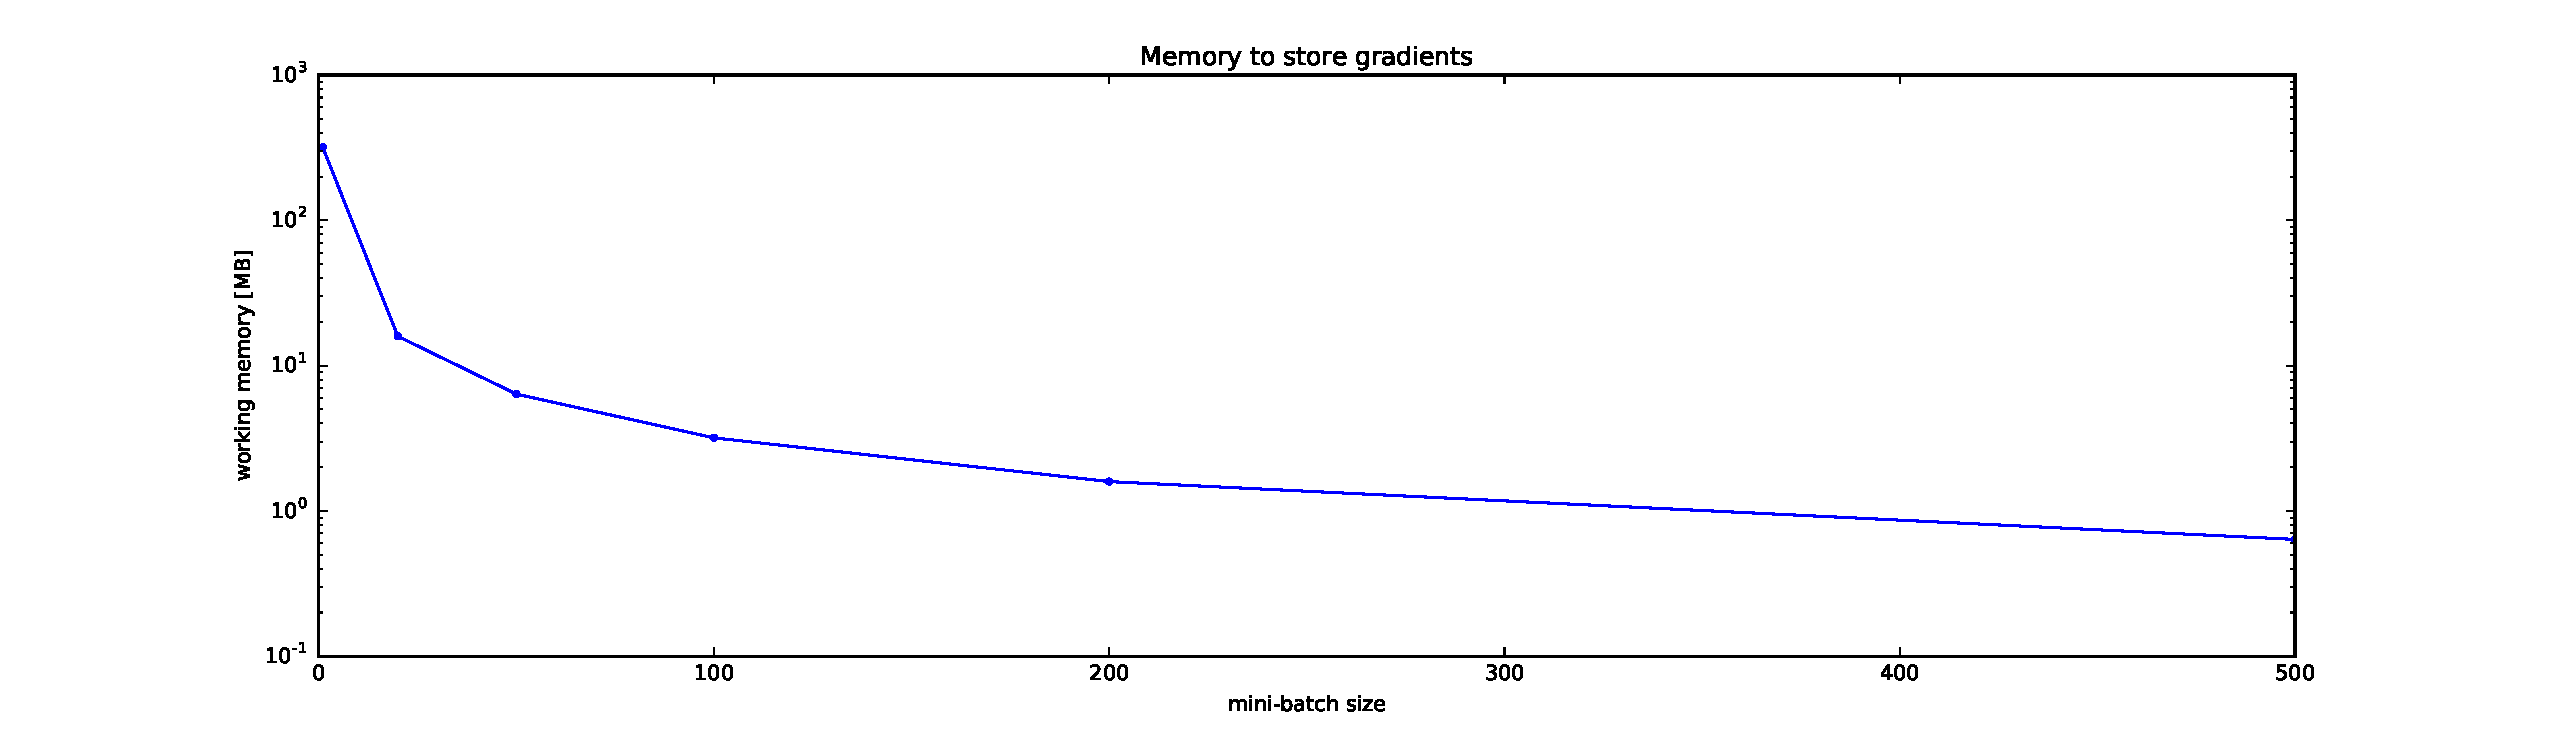
\includegraphics[height=3cm,width=0.45\columnwidth]{memory}}
	\hspace{0pt}
	\subfigure{
		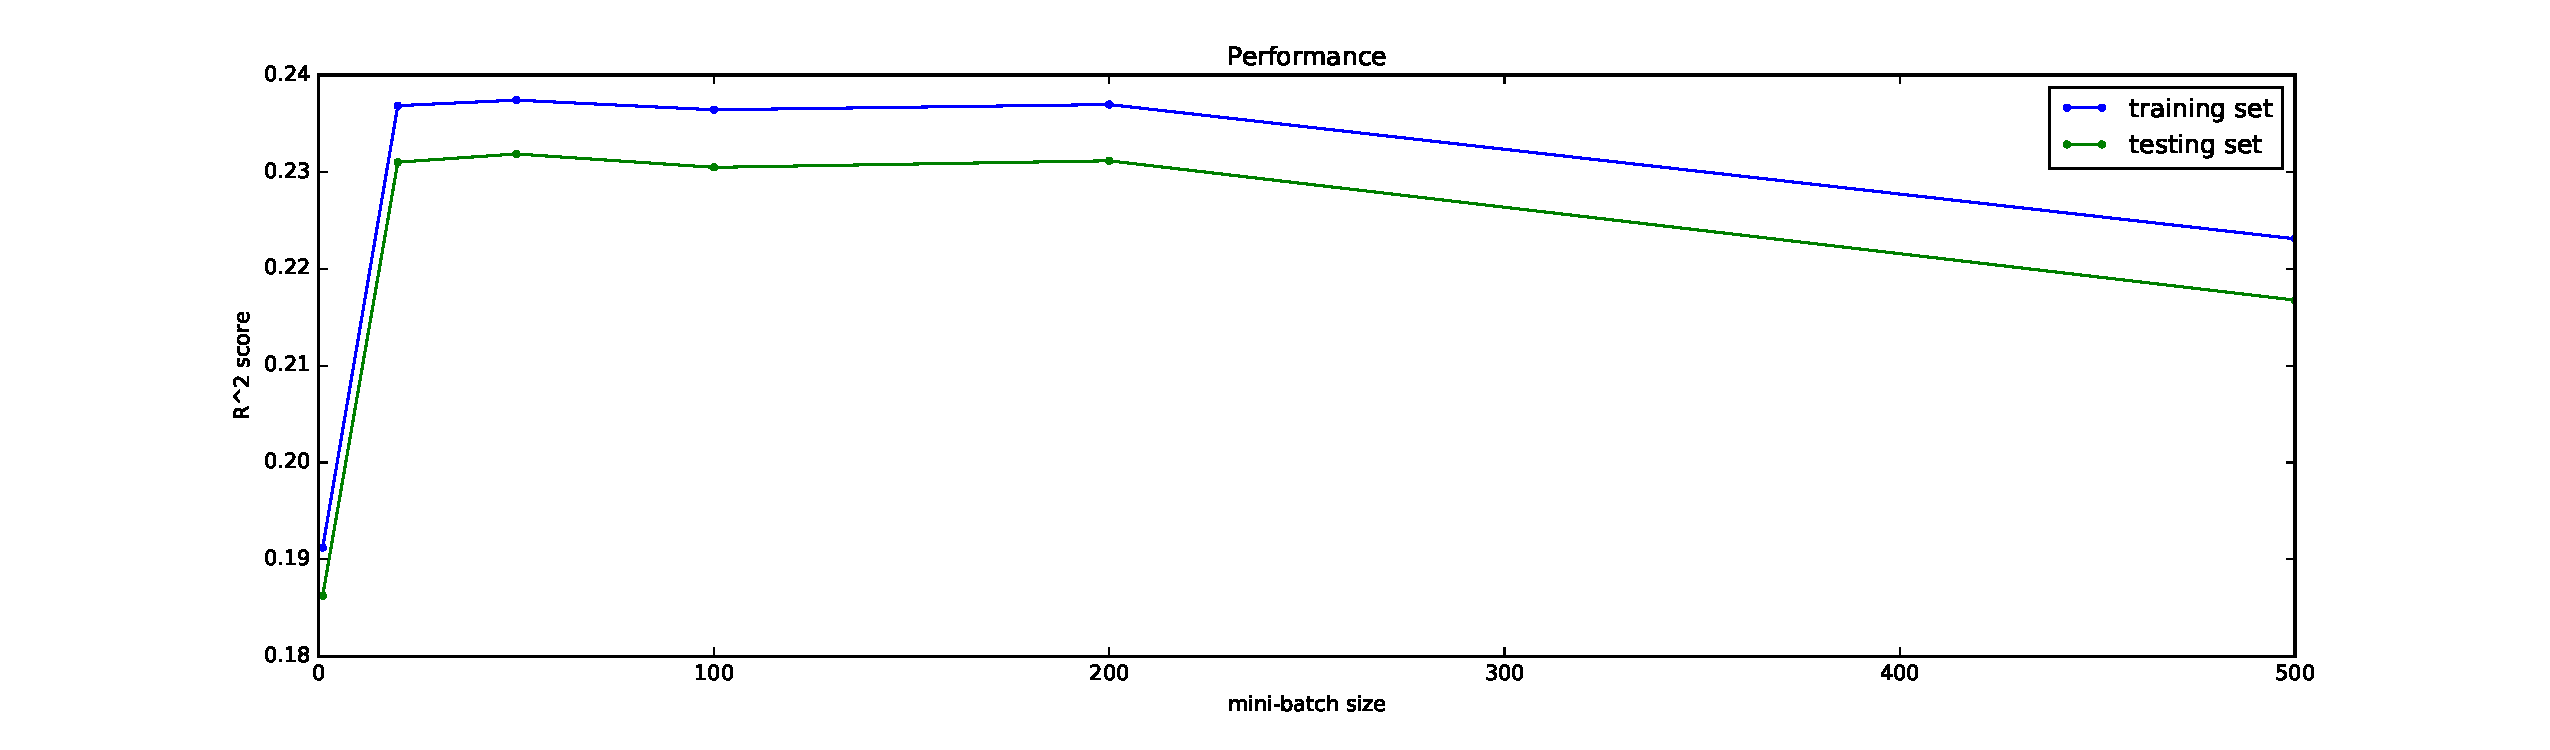
\includegraphics[height=3cm,width=0.45\columnwidth]{r2_score}}
	\\
	\subfigure{
		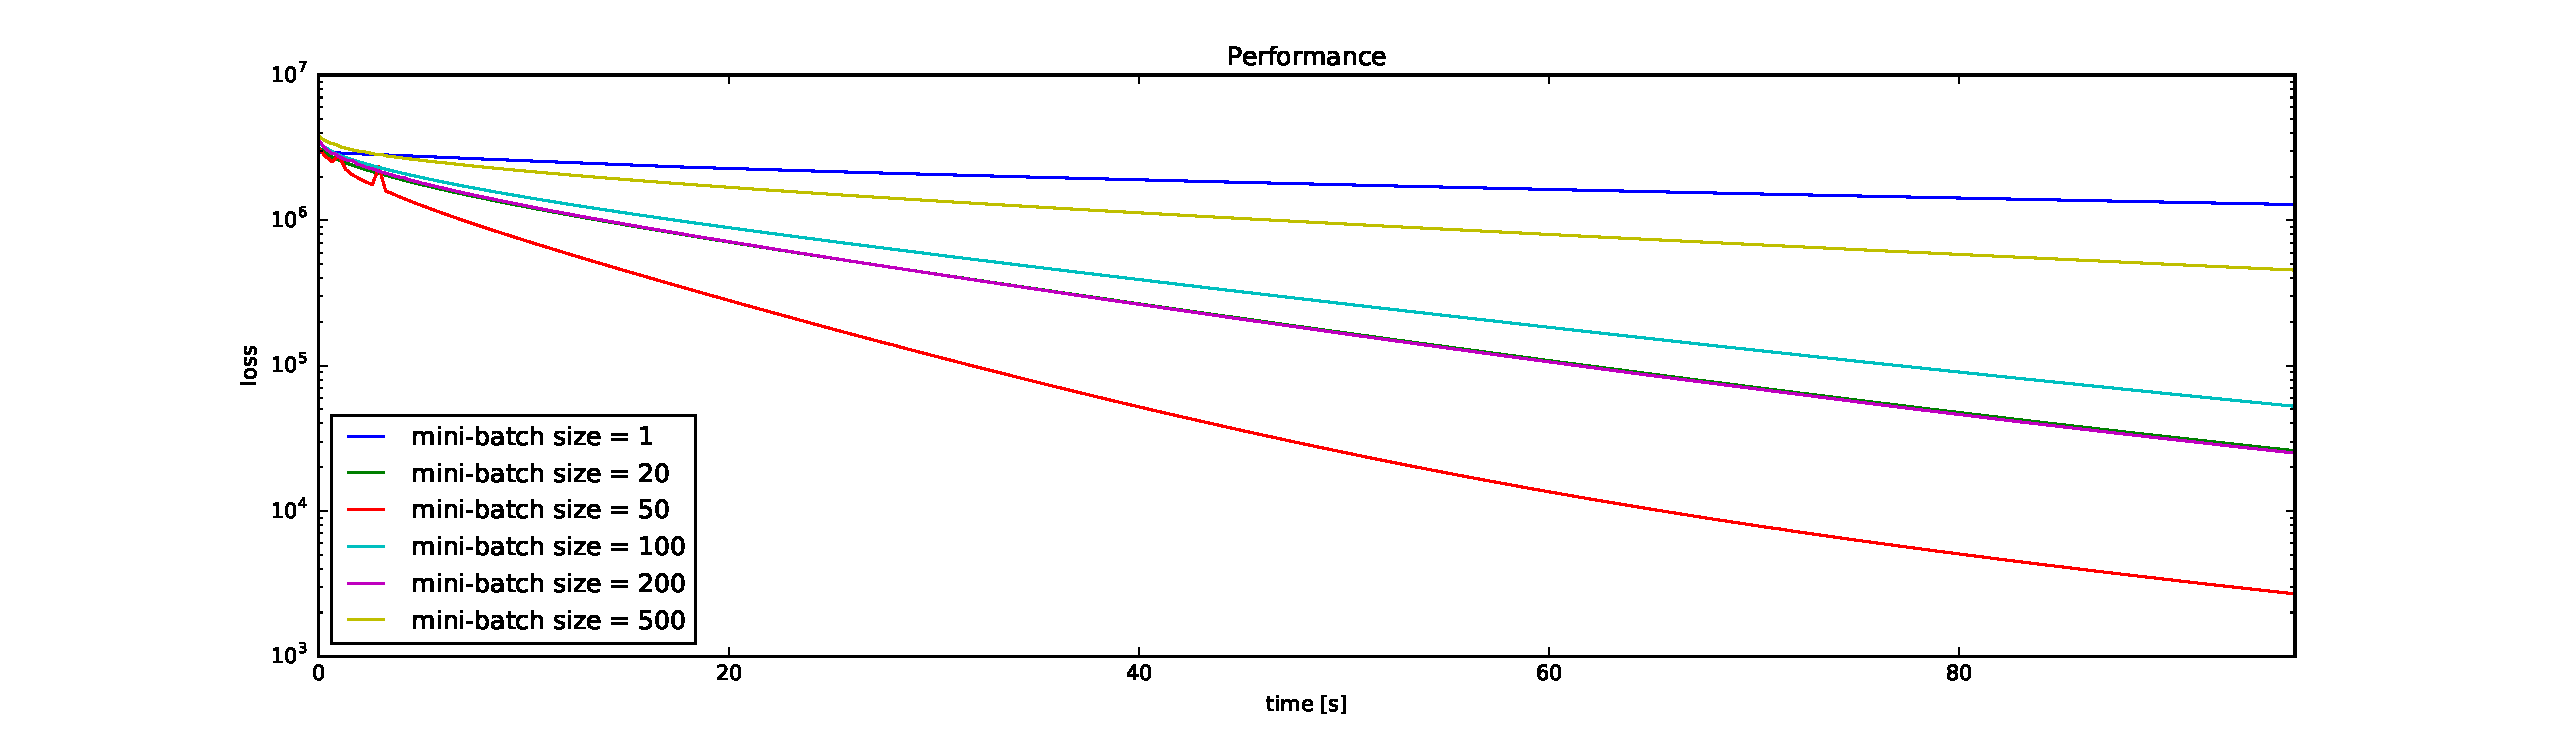
\includegraphics[height=4cm,width=0.7\columnwidth]{perf}}
	\caption{Performance evaluation of mini-batch SAGA.}
	\label{eval_saga_mb}
\end{figure}

\end{frame}

\section{Distributed SAGA}

\begin{frame}{The First Approach}
	\centering
	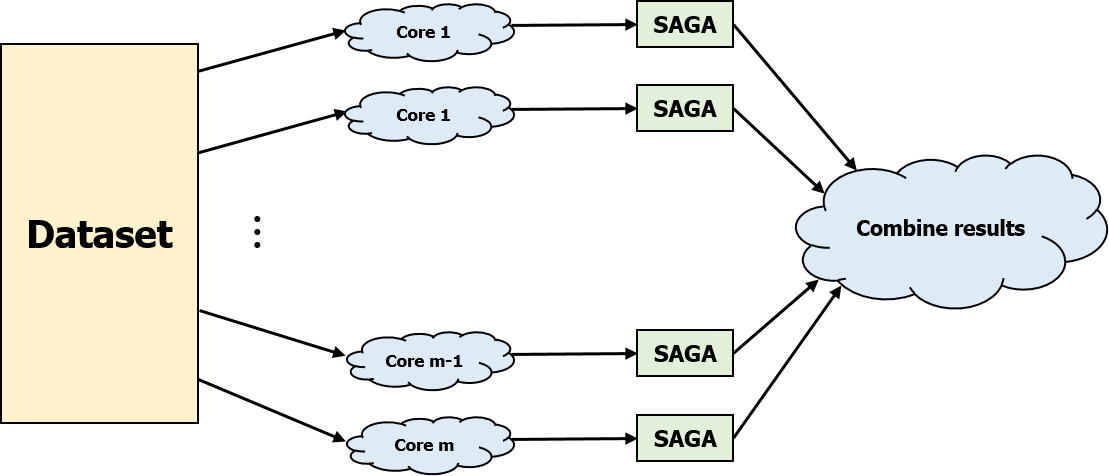
\includegraphics[scale=0.35]{Picture1.png}
	\visible<2>
	{
		\medskip
		\medskip
		\centering
		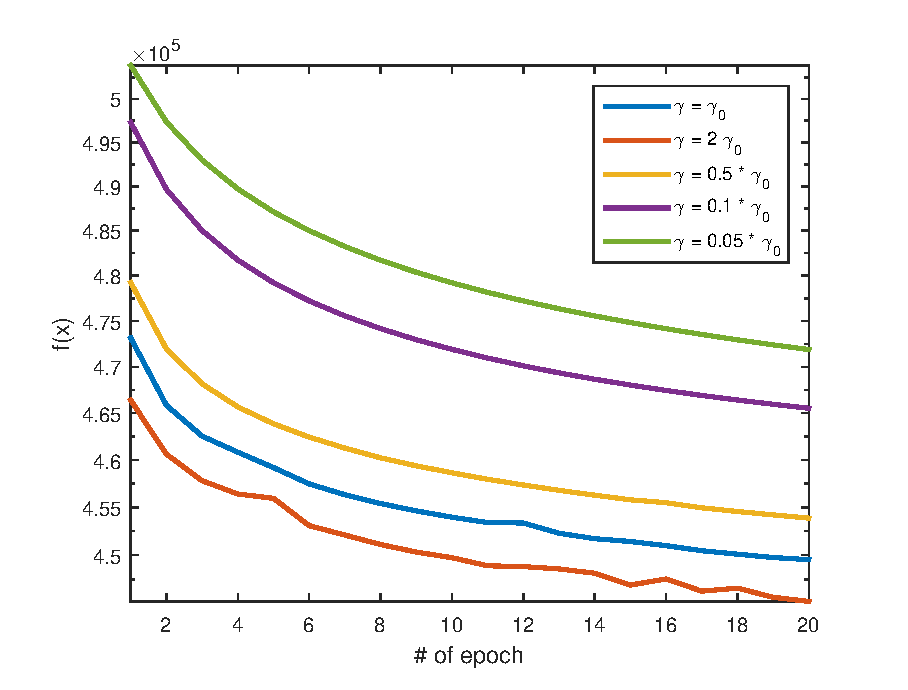
\includegraphics[scale=0.5]{distributed1.eps} 
	}
\end{frame}

\begin{frame}{The Second Approach}
	\centering
	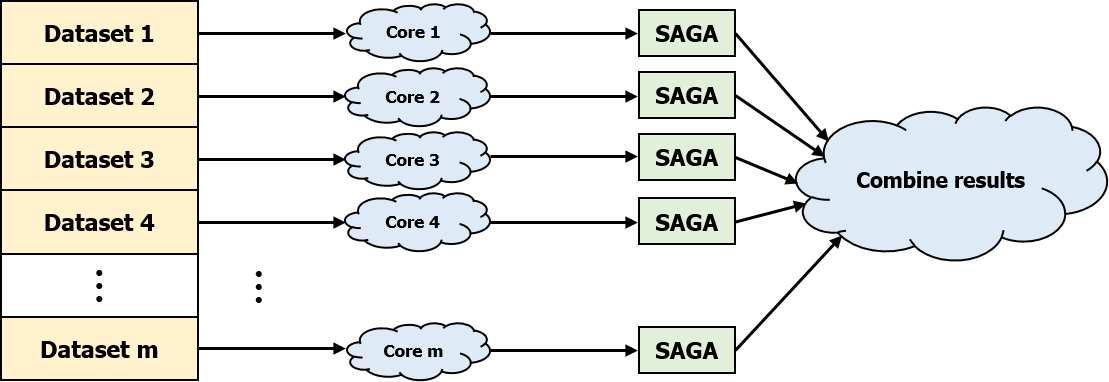
\includegraphics[scale=0.35]{Picture2.png}
	\visible<2->
	{
		\medskip
		\medskip
		\centering
		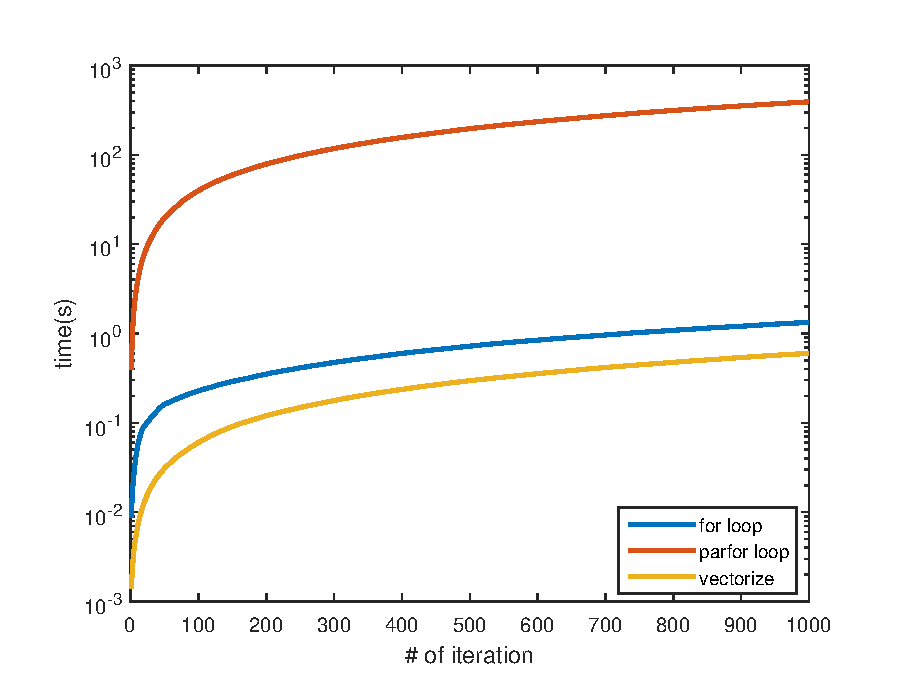
\includegraphics[scale=0.5]{distributed2.eps} 
	}
\end{frame}

\begin{frame}{The Second Approach}
	\centering
	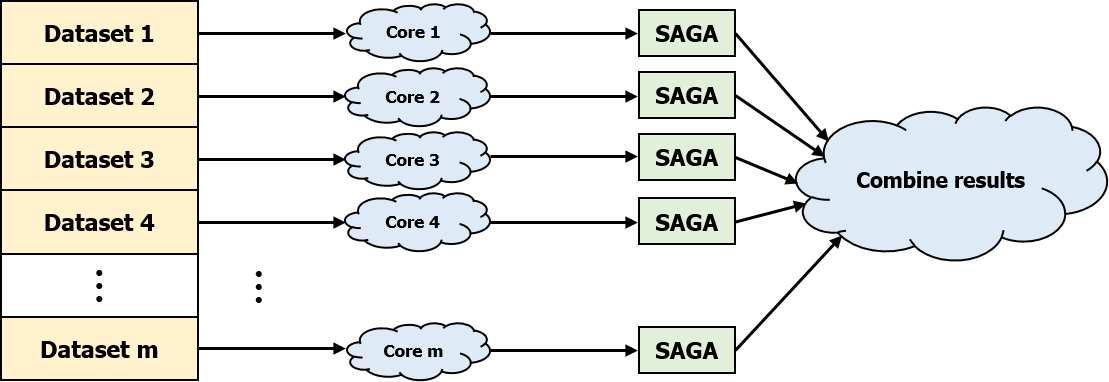
\includegraphics[scale=0.35]{Picture2.png}
	
	\centering
	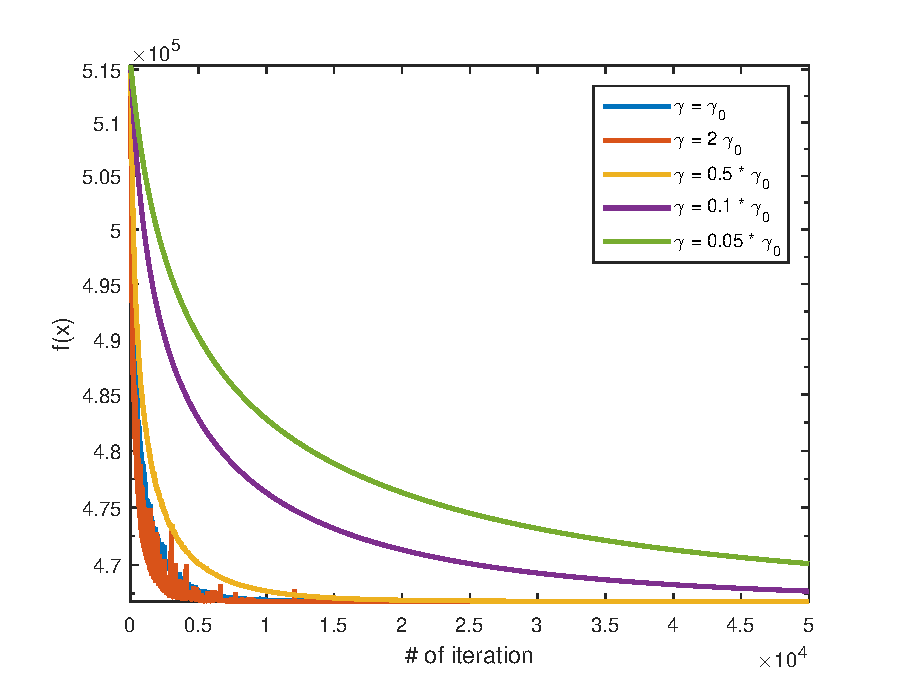
\includegraphics[scale=0.5]{distributed3.eps} 
\end{frame}

\begin{frame}{Compare First and Second Approach}
	\medskip
	\medskip
	\medskip
	\medskip
	\medskip
	\medskip
	\medskip
	\centering
	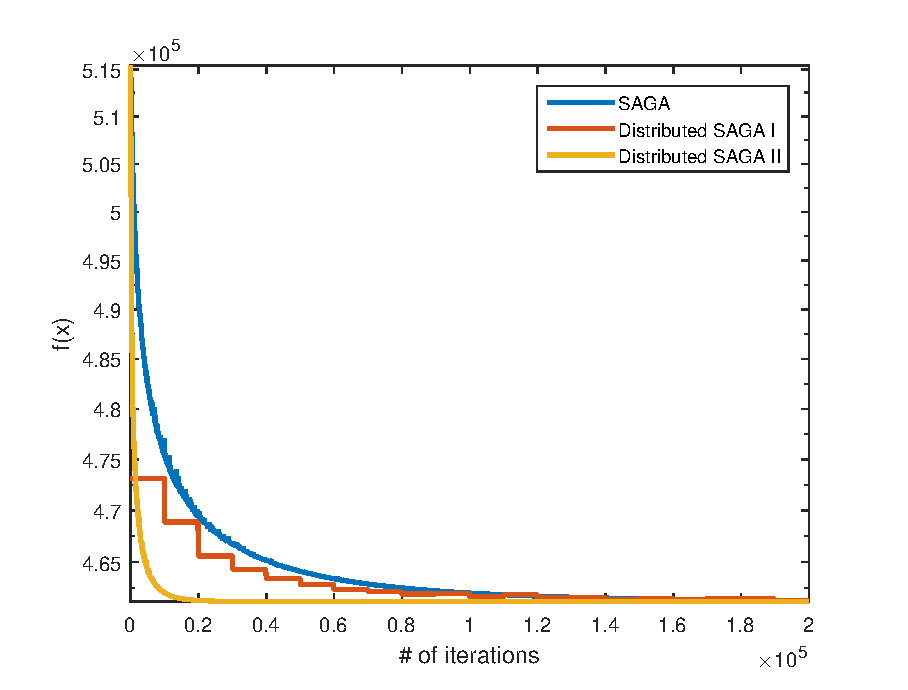
\includegraphics[scale=0.4]{compare.eps}
	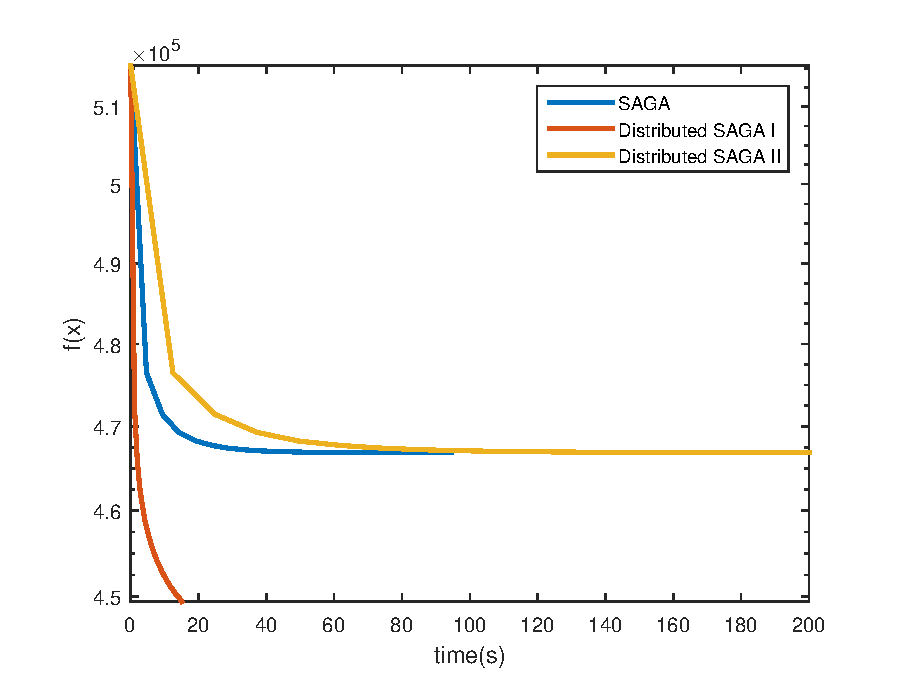
\includegraphics[scale=0.4]{compare2.eps} 
\end{frame}


\end{document}
